\section{Métodos e Algoritmos para Recuperação da Informação Musical} \label{cap:metodos}

A análise da informação musical para sua representação apresenta complexidades, pois exige diferentes técnicas de extração de informações para distintas formas de apresentação \cite{downie2003}.

Um dado musical geralmente é representado por um conjunto de características extraídas do conteúdo da música. Isto porque dados musicais são basicamente arranjos multidimensionais de valores derivados de vários sensores, que é uma representação limitada para definir a semântica do dado. Neste sentido, dados complexos raramente são comparados diretamente. Em vez disso, o conteúdo do dado (ou uma faceta do conteúdo) é analisado por meio de algoritmos especializados de análise, extraindo um conjunto de características que descrevem numericamente o dado \cite{kaster2012}. Desta forma, as aplicações que lidam com dados complexos, como dados musicais, requerem a realização de consultas por similaridade, ou seja, consultas que realizam busca por objetos da base que sejam similares a um objeto de consulta, de acordo com uma certa medida de similaridade \cite{barioni2006}.

A Sociedade Internacional de Recuperação da Informação Musical (ISMIR\footnote{https://transactions.ismir.net/}, na sigla em inglês) abriga, durante sua conferência anual, o MIREX\footnote{http://www.music-ir.org/mirex/wiki/MIREX\_HOME}, com o objetivo de estabelecer métodos para a avaliação e comparação das aplicações atuais de recuperação musical. Nesta espécie de competição, pesquisadores inscrevem algoritmos que realizam diferentes tarefas da área de recuperação da informação musical, como classificação automática de gênero musical, identificação automática da pulsação, extração de melodia a partir de arquivos áudio, entre outros.

\begin{figure}[!ht]
   \centering
   \caption{Representação do modelo de recuperação de informação musical} 
   \label{fig:modeloRecInfo} 
   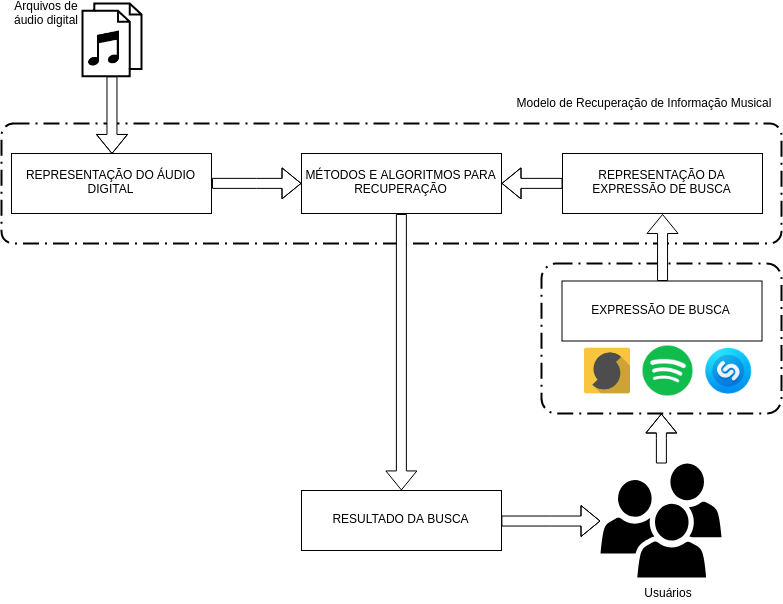
\includegraphics[scale=0.30]{figuras/modeloRecInfo.png}
   \\Fonte: \cite{ferreira2015}, adaptado pela autora
\end{figure}

Um sistema de recuperação de informação musical atua, portanto, como um ambiente mediador da comunicação entre as necessidades informacionais dos usuários e o conjunto de arquivos de áudio. Na Figura \ref{fig:modeloRecInfo} é possível compreender melhor o processo de recuperação de informação. Dadas as características de um sinal de áudio, pode-se definir métricas de similaridade para comparar músicas. Embora exista uma grande variedade de funções de distância disponível na literatura, não existe um método que determine, de um modo geral, qual deve ser a melhor função de distância a ser utilizada em cada caso. A escolha ou definição de uma função de distância é uma tarefa que depende muito da análise das características específicas do domínio dos dados a serem manipulados \cite{barioni2006}.

O foco deste trabalho não é aprofundar o conhecimento nos métodos e algoritmos utilizados para recuperação da informação musical. Assim sendo, os principais métodos e algoritmos disponíveis na literatura são descritos aqui de forma breve.

\subsection{Audio Fingerprint} \label{subsec:audioFingerprint}
\textit{Audio Fingerprint} é como uma assinatura única de uma música, contendo um sumário de suas características que resume uma gravação de áudio. \cite{cano2005} que definem que uma \textit{fingerprint} de áudio é um resumo digital, que pode ser utilizado para identificar uma amostra ou localizar rapidamente itens semelhantes em uma base de dados de áudio, independente do nível de compressão, distorção ou interferência no canal de transmissão. A questão fundamental é como fazer a comparação eficiente do áudio desconhecido contra os possíveis milhões de \textit{fingerprints} \cite{cano2005}.

\subsection{Classificação} \label{subsec:classificacao}
Classificação é a tarefa de aprender uma função alvo \textbf{\({f}\)} que mapeie cada conjunto de atributos \textbf{\({x}\)} para um dos rótulos de classes \textbf{\({y}\)} pré-determinados \cite{pang2009}. A função alvo também é conhecida como modelo de classificação e, segundo \cite{pang2009}, pode ser classificada de duas formas: Modelagem Descritiva e Modelagem Preditiva; E os métodos de classificação podem ser divididos de duas formas: classificadores \textit{eager} (espertos) e classificadores \textit{lazy} (preguiçosos). Técnicas de classificação são mais apropriadas para prever ou descrever conjuntos de dados com categorias nominais ou binárias, sendo menos efetivas para categorias ordinais.

\subsection{Clustering}\label{subsec:clustering}
A formação de agrupamentos (ou \textit{clustering}) divide os dados em grupos (\textit{clusters}) que tenham significado, sejam úteis, ou ambas as coisas. Se \textit{clusters} com significados forem o objetivo, então os \textit{clusters} devem capturar a estrutura natural dos dados. O objetivo é que os objetos dentro de um \textit{cluster} sejam semelhantes (ou relacionados) entre si e diferentes de (ou não relacionados aos) objetos de outros \textit{clusters}. Quanto maior a semelhança (ou homegeneidade) dentro de um \textit{cluster} e maior a diferença entre \textit{clusters}, melhor ou mais distinto será o agrupamento \cite{pang2009}.

\subsection{Dynamic Time Warping} \label{subsec:dtw}
O \textit{Dynamic Time Warping} (DTW) \cite{keogh2004} é uma técnica que permite definir uma métrica entre séries temporais, como por exemplo, características de áudio. Seu uso é inviável em grandes conjuntos de dados. Por este motivo, diversas técnicas de indexação específicas para esse algoritmo foram propostas para a tarefa de busca por similaridade, tais como \textit{lower bound} e \textit{early abandoning}. Com essas técnicas, é possível encontrar os vizinhos mais próximos de uma dada subsequência em uma quantidade massiva de séries temporais. Informações mais detalhadas podem ser consultadas em \cite{mizutani2006}, \cite{kruskal1983} e \cite{juang1991}.

\subsection{Indexação}\label{subsec:indexacao}
Estruturas de indexação (uma descrição sobre essas estruturas pode ser encontrada em \cite{garciaMolina2002}) são normalmente fornecidas pelos SGBDs. A idéia básica dessas estruturas consiste na escolha de um objeto arbitrário central e na aplicação de uma função de distância para dividir os demais objetos em vários subconjuntos. Dessa maneira, uma estrutura de indexação é construída executando-se esse mesmo procedimento, recursivamente, para cada subconjunto não vazio \cite{barioni2006}. Assim como a \textit{Slim-tree}, na literatura podem ser encontradas outros métodos aplicados à indexação de dados musicais, são a \textit{VP-tree} (\textit{Vantage Point tree}) \cite{yanilos1993}, a \textit{MVP-tree} (\textit{Multi-Vantage Point tree}) \cite{bozkaya1997}, a GNAT (\textit{Geometric Near-neighbor Access Tree}) \cite{brin1995}, a \textit{M-tree} \cite{ciaccia1997}, \textit{Família-Omni} e a \textit{DBM-tree} \cite{filho2001, vieira2004}, a \textit{n-grams} \cite{downie1999} e o \textit{Vantage Indexing Method} \cite{typke2003}.

\subsection{Medidas de Similaridade} \label{subsec:medidas-similaridade}
A semelhança entre dois objetos é uma medida numérica do grau no qual os dois objetos se parecem. A diferença, ou dissimilaridade, entre dois objetos é uma medida númerica do grau no qual os dois objetos são diferentes. Frequentemente, o termo distância é usado como sinônimo de diferença, embora, muitas vezes seja usado para se referir a uma classe especial de diferenças. Similaridade e distância são importantes pois são utilizadas por inúmeras técnicas de mineração de dados, como \textit{clustering} (ver subseção \ref{subsec:clustering}) e classificação (ver subseção \ref{subsec:classificacao}). Quanto menor o valor desta distância, mais semelhantes serão os objetos e eles tenderão a ficar no mesmo cluster. Quanto maior a distância, menos similares serão os objetos e, em consequência, eles deverão estar em grupos distintos.

\subsection{Query by Humming} \label{subsec:qbh}
A tarefa de busca musical a partir de um trecho de música cantada ou cantarolada pelo usuário passou a ser conhecida na literatura como \textit{query by humming}, ou QBH. Trata-se de um sistema capaz de reconhecer música pelo \textit{casamento aproximado} de cadeias de caracteres. \cite{ghias1995}, autores do projeto, aplicaram o conceito de \textit{contorno melódico}, ou seja, a forma natural como nós percebemos a música. Segundo \cite{santos2011}, existem dois principais interesses em QBH: Primeiramente, permitir ao usuário identificar uma música da qual não conheça (ou lembre de) qualquer metadado associado (autor, álbum, título da música, entre outros). Em segundo, é dispor de uma maneira mais natural para consultar coleções de músicas digitais armazenadas principalmente em dispositivos portáteis.

\subsection{Recuperação por Conteúdo} \label{subsec:rpc}
A recuperação por conteúdo aplica-se a vários tipos de dados, inclusive música, e com o aumento da disponibilização de coleções de áudio digitais, se tornou importante permitir o gerenciamento automático desses tipos de dados por meio da utilização de metadados (como título, álbum e gênero da música). Assim, várias técnicas de extração de metadados foram desenvolvidas, sendo algumas delas especialmente adequadas à recuperação de música por conteúdo. As técnicas baseadas em busca por conteúdo utilizam metadados extraídos automaticamente dos dados musicais para representar e indexar as informações embutidas nos áudios digitais. O conjunto de metadados extraídos é chamado de \textit{vetor de características} \cite{tzanetakis2002}. E as operações de comparação entre dados musicais utilizam os vetores de características para medir a similaridade do conteúdo presente nos dados que eles representam.

\subsection{Spectral Modeling Synthesis} \label{subsec:sms}
\textit{Spectral Modeling Synthesis} (SMS), ou na sua tradução, Síntese de Modelagem Espectral, é uma abordagem de modelagem acústica para voz e outros sinais musicais. Ele considera os sons como uma combinação de conteúdo harmônico e conteúdo de ruído. Os componentes harmônicos são identificados com base em picos no espectro de freqüência do sinal, normalmente encontrados pela transformada de Fourier de curta duração (FFT). O sinal que permanece após a remoção dos componentes espectrais, por vezes referido como residual, é modelado como ruído branco passado através de um filtro que varia no tempo. A saída do modelo, então, são as frequências e níveis dos componentes harmônicos detectados e os coeficientes do filtro que variam no tempo. Essas técnicas podem ser usadas para aplicações de síntese, processamento e codificação, enquanto alguns dos resultados intermediários também podem ser aplicados a outros problemas relacionados à música, como separação de fontes sonoras, acústica musical, percepção musical ou análise de desempenho. Informações mais detalhadas sobre a técnica pode ser encontradas em \cite{serra1990}.

\subsection{Visualização} \label{subsec:visualizacao}
Visualização de dados musicais é a exibição na forma de um gráfico ou tabela. Uma visualização bem sucedida requer que os dados sejam convertidos em um formato visual de modo que as carcterísticas dos mesmos e dos relacionamentos entre itens de dados possam ser analisados ou reportados. O objetivo da visualização é a interpretação da informação visualizada por uma pessoa e a formação de um modelo mental das informações \cite{pang2009}.
